\documentclass[10pt,conference,onecolumn,compsoc]{IEEEtran}

\usepackage{hyperref}
\usepackage{enumitem}
\setlist[itemize]{leftmargin=3 cm}
\setlist[enumerate]{leftmargin=3cm}

\ifCLASSOPTIONcompsoc

 \usepackage[nocompress]{cite}
\else
  % normal IEEE
  \usepackage{cite}
\fi


\ifCLASSINFOpdf
   \usepackage[pdftex]{graphicx}

\else

\fi



\begin{document}
%
\title{2D Top-Down Shooter \\ for UTM CSCI 352 Spring 2017}

\author{Cole Davis and Mel Howard}

\IEEEtitleabstractindextext{%
\begin{abstract}
The proposed game will be a multi-level top-down shooter. The player character will use projectiles to defeat increasing hordes of enemies as he or she progresses through the game. The player progresses by defeating a predetermined number of enemies, allowing them to move to the next location.
\end{abstract}
}


% make the title area
\maketitle


\IEEEdisplaynontitleabstractindextext

\IEEEpeerreviewmaketitle



\section{Introduction}
The game will let users create a player and control it vertically and horizontally using the WASD keyboard keys. The player will travel to different locations, then fight and kill enemies with projectiles from a ranged weapon. This game's target audience is college aged programmers (specifically CS majors), and any retro game enthusiasts. We hope the target audience will at first be engaged, and then extremely frustrated.


\subsection{Background}
A top-down shooter is a game where the user controls his or her character from a birds eye view of their avatar and the surroundings.

\subsection{Challenges}
One of the most daunting challenges of the proposed game is animating the player avatar and enemies in WPF.
Another issue we anticipate is updating the player score or "kill count" as the player shoots at enemies.

\section{Scope}


The project will be done when:
	\begin{itemize}
		\item the user can create a player avatar
		\item move avatar around rooms using keyboard controls
		\item projectiles hitting enemies are registered, "kill" enemy, and update score
		\item there are a minimum of six locations/rooms/levels
		\item levels spawn a predetermined (and increasing) number of enemies
		\item final location has a "boss monster" whose defeat ends the game
	\end{itemize} 
Stretch Goals:
	\begin{itemize}
		\item enemies can shoot back at player
		\item player can collect items/power-ups
		\item local cooperative play
		\item perpetual game record - save game
	\end{itemize}

\subsection{Requirements}
As part of fleshing out the scope of your requirements, you'll also need to keep in mind both your functional and non-functional requirements.  These should be listed, and explained in detail as necessary.  Use this area to explain how you gathered these requirements.

\subsubsection{Functional}
\begin{itemize}
\item User needs to have a private shopping cart -- this cannot be shared between users, and needs to maintain state across subsequent visits to the site
\item Users need to have website accounts -- this will help track recent purchases, keep shopping cart records, etc.
\item You'll need more than 2 of these...
\end{itemize}

\subsubsection{Non-Functional}
\begin{itemize}
\item Security -- user credentials must be encrypted on disk, users should be able to reset their passwords if forgotten
\item you'll typically have fewer non-functional than functional requirements
\end{itemize}

\subsection{Use Cases}
This subsection is arguably part of how you define your project scope (why it is in the Scope section...).  In a traditional Waterfall approach, as part of your requirements gathering phase (what does the product actually \emph{need} to do?), you will typically sit down with a user to develop use cases.

You should have a table listing all use cases discussed in the document, the ID is just the order it is listed in, the name should be indicative of what should happen, the primary actor is typically most important in an application where you may have different levels of users (think admin vs normal user), complexity is a best-guess on your part as to how hard it should be.  A lower number in priority indicates that it needs to happen sooner rather than later.  A sample table, or Use Case Index can be seen in Table \ref{tab:useCaseIndex}.


\begin{itemize}
\item[Use Case Number:] 1
\item[Use Case Name:] Add item to cart
\item[Description:] A shopper on our site has identified an item they wish to buy.  They will click on a ``Add to Cart" button.  This will kick off a process to add one instance of the item to their cart.
\end{itemize}

You will then go on to (minimally) discuss a basic flow for the process:

\begin{enumerate}
\item User navigates to page listing desired item
\item User left-clicks on ``Add to Cart" button.
\item User cart is updated to reflect the new item, this also updates the current total.
\item[Termination Outcome:] The user now has a single instance of the item in their cart.
\end{enumerate}

You may need to also add in any alternative flows:

Alternative: Item already exists in the cart
\begin{enumerate}
\item User navigates to page listing desired item
\item User left-clicks on ``Add to Cart" button.
\item User cart is updated to reflect the new item, showing that one more instance of the existing item has been added.  This also updates the current total.
\item[Termination Outcome:] The user now has multiple instances of the item in their cart.
\end{enumerate}

You will often also need to include pictures or diagrams.  It is quite common to see use-case diagrams in such write-ups.  To properly reference an image, you will need to use the \texttt{figure} environment and will need to reference it in your text (via the \texttt{ref} command) (see Figure \ref{cat1}).  NOTE: this is not a use case diagram, but a kitten.

After fully describing a use case, it is time to move on to the next use case:

\begin{itemize}
\item[Use Case Number:] 2
\item[Use Case Name:] Checkout
\item[Description:] A shopper on our site has finished shopping.  They will click on a ``Checkout" button.  This will kick off a process to calculate cart total, any taxes, shipping rates, and collect payment from the shopper.

\end{itemize}

You will then need to continue to flesh out all use cases you have identified for your project.

\begin{figure}[ht!]
%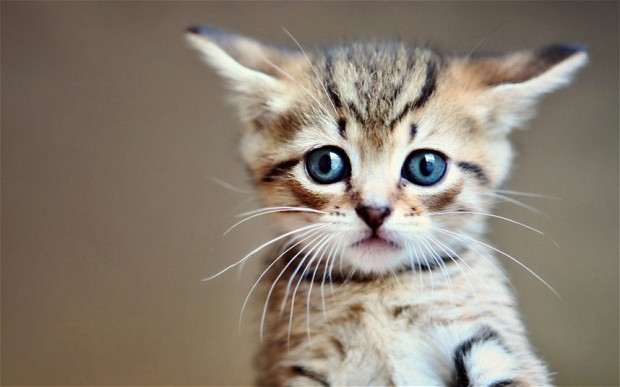
\includegraphics[height=250px, width=350px]{cat1.jpg}
\caption{First picture, this is a kitten, not a use case diagram}
%\label{cat1}
\end{figure}

\subsection{Interface Mockups}
At first, this will largely be completely made up, as you get further along in your project, and closer to a final product, this will typically become simple screenshots of your running application.

In this subsection, you will be showing what the screen should look like as the user moves through various use cases (make sure to tie the interface mockups back to the specific use cases they illustrate).



\section{Project Timeline}
Go back to your notes and look up a typical project development life cycle for the Waterfall approach.  How will you follow this life cycle over the remainder of this semester?  This will usually involve a chart showing your proposed timeline, with specific milestones plotted out.  Make sure you have deliverable dates from the course schedule listed, with a plan to meet them (NOTE: these are generally optimistic deadlines).

\section{Project Structure}
At first, this will be a little empty (it will need to be filled in by the time you turn in your final report).  This is your chance to discuss all of your design decisions (consider this the README's big brother).

\subsection{UML Outline}
Show the full structure of your program.  Make sure to keep on updating this section as your project evolves (you often start out with one plan, but end up modifying things as you move along).  As a note, while Dia fails miserably at generating pdfs (probably my fault), I have had much success with png files.  Make sure to wrap your images in a \texttt{figure} environment, and to reference with the \texttt{ref} command.  For example, see Figure %\ref{cat2}.

%\begin{figure}[ht!]
%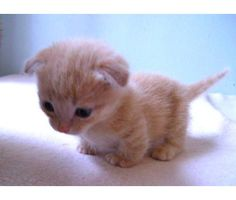
\includegraphics[scale=1.5]{cat2.jpg}
%caption{Your figures should be in the \emph{figure} environment, and have captions.  Should %also be of diagrams pertaining to your project, not random internet kittens}
%\label{cat2}
%\end{figure}


\subsection{Design Patterns Used}
Make sure to actually use at least 2 design patterns from this class.  This is not normally part of such documentation, but largely just specific to this class -- I want to see you use the patterns!


\section{Results}
This section will start out a little vague, but it should grow as your project evolves.  With each deliverable you hand in, give me a final summary of where your project stands.  By the end, this should be a reflective section discussing how many of your original goals you managed to attain/how many desired use cases you implemented/how many extra features you added.

\subsection{Future Work}
Where are you going next with your project?
For early deliverables, what are your next steps?  (HINT: you will typically want to look back at your timeline and evaluate: did you meet your expected goals?  Are you ahead of schedule?  Did you decide to shift gears and implement a new feature?)
By the end, what do you plan on doing with this project?  Will you try to sell it?  Set it on fire?  Link to it on your resume and forget it exists?




\begin{thebibliography}{1}

\bibitem{IEEEhowto:kopka}
H.~Kopka and P.~W. Daly, \emph{A Guide to \LaTeX}, 3rd~ed.\hskip 1em plus
  0.5em minus 0.4em\relax Harlow, England: Addison-Wesley, 1999.
\end{thebibliography}


\begin{IEEEbiography}{Michael Shell}
Biography text here.
\end{IEEEbiography}

% if you will not have a photo at all:
\begin{IEEEbiographynophoto}{John Doe}
Biography text here.
\end{IEEEbiographynophoto}

% insert where needed to balance the two columns on the last page with
% biographies
%\newpage

\begin{IEEEbiographynophoto}{Jane Doe}
Biography text here.
\end{IEEEbiographynophoto}

% You can push biographies down or up by placing
% a \vfill before or after them. The appropriate
% use of \vfill depends on what kind of text is
% on the last page and whether or not the columns
% are being equalized.

%\vfill

% Can be used to pull up biographies so that the bottom of the last one
% is flush with the other column.
%\enlargethispage{-5in}



% that's all folks
\end{document}


